\documentclass{beamer}
\usepackage{float}
\title{A Tutorial on EM for HMM}
\subtitle{A try on YuChen's \LaTeX~Beamer template}
\author{Goose He}
\date{March 2013}

\usetheme{CambridgeUK}

\begin{document}

\begin{frame}
\titlepage
\end{frame}

\begin{frame}

\begin{abstract}
A Tutorial on the Expectation Maximization(EM) Alogrithm for Hidden Markov Model with single Guassian. Nearly all material of this tutorial is from KaiYu's thesis 'Adaptive Training for Large Vocabulary Continuous Speech Recognition'.\\
If you have a problem during the presentation, please \alert{ask directly}. I hope that I didn't make a mistake and at the end everyone will understand as much as I do.

\end{abstract}

\end{frame}

\begin{frame}
\frametitle{A quick introduction to MLE}
We use a Guassian distrubution 
\begin{equation}
\mathcal{N}(x | \mu, \Sigma) = \frac{1}{(2\pi)^{D/2}}\frac{1}{|\Sigma|^{1/2}}exp\{-\frac{1}{2}(x-\mu)^T\Sigma^{-1}(x-\mu)\}
\end{equation}
We want to estimate the parameters $\mu$ and $\Sigma$, however, we only have some observance $x_1, x_2, ... , x_N$ that are drawn independently from the distribution.
\end{frame}

\begin{frame}
\frametitle{A quick introduction to MLE}
MLE means maximum likelyhood estimation. We maximize $\prod_i \mathcal{N}(x_i|\mu, \Sigma)$. This is equivalent to maximize the log likelyhood function.(Note that now I only consider $\mu$, so others are considered constant and thrown away)
\begin{equation}
M(\mu, \Sigma) = log\prod_i \mathcal{N}(x_i|\mu, \Sigma) = \sum_i(-\frac{1}{2}(x_i-\mu)^T\Sigma^{-1}(x_i-\mu))
\end{equation}
To maximize with respect to $\mu$,we set $\frac{\partial M}{\partial \mu}=0$, that is
\begin{equation}
\begin{split}
\sum_{i=1}^{N}\Sigma^{-1}(x_i-\mu) = 0 \\
\hat{\mu}_{ML}=\frac{1}{N}\sum_{i=1}^{N}x_i
\end{split}
\end{equation}
\end{frame}
\begin{frame}
For maximizing with respect to $\Sigma$,I encourage readers to PRML \$2.3.4.
\end{frame}

\begin{frame}
\frametitle{A quick introduction to Hidden Markov Model}
\begin{figure}
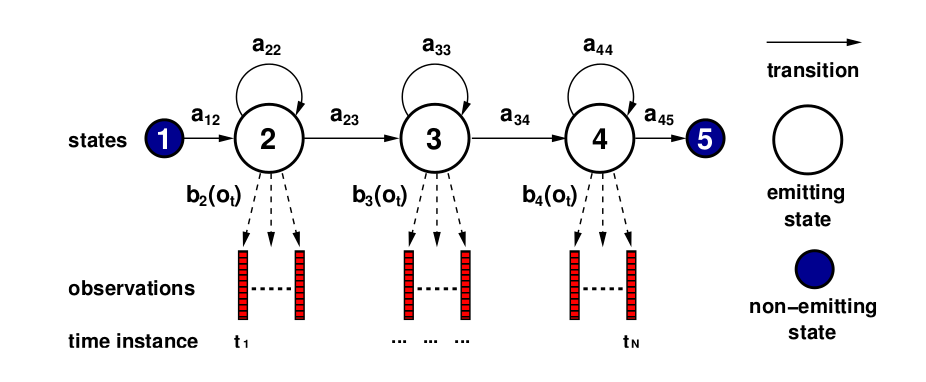
\includegraphics[width=240pt]{HMM.png}
\end{figure}
We use a HMM to model a \emph{context dependent phone}. $a_{ij}$ is the state transition probability. $b(o)$ is a single Guassian distribution that models the observance that this state.\\
We call $O=(o_1,o_2,...,o_T)$ the observance of a HMM, and $w = (w_1,w_2,...,w_T)$ the hidden state sequence.
\end{frame}

\begin{frame}
\frametitle{HMM for a context dependent phone}
\begin{figure}
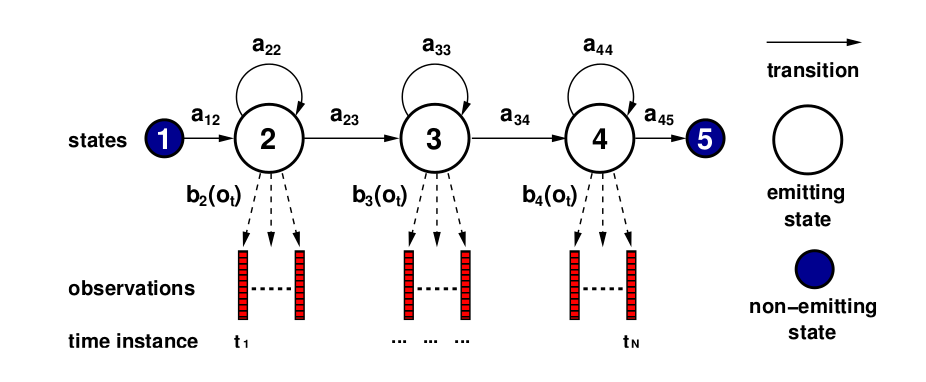
\includegraphics[width=240pt]{HMM.png}
\end{figure}
For example, If we want to model the $wa$ in $ae + wa + n + t$ for 'I want'. We create a HMM called 'ae + wa + n', where the 'wa' is called the center phone. State 2 for ae, State 3 for wa, and State 4 for n.
\end{frame}


\begin{frame}
\frametitle{A quick introduction to Hidden Markov Model}
\framesubtitle{composite HMM}
\begin{figure}
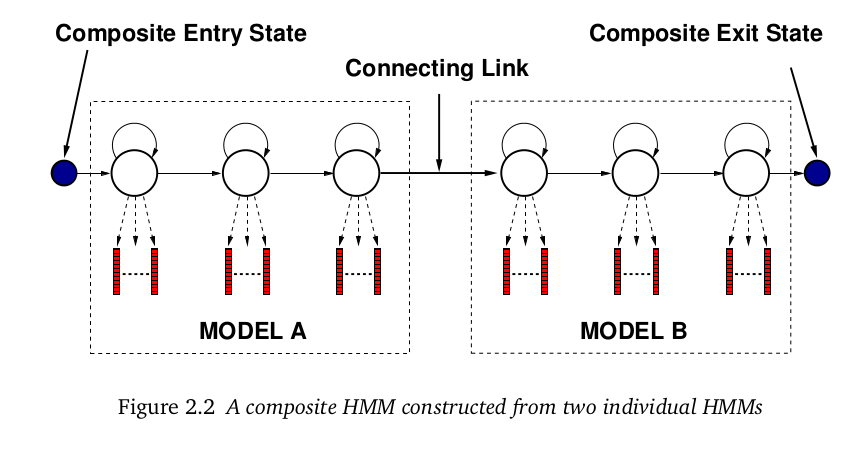
\includegraphics[width=240pt]{composite-HMM.png}
\end{figure}
We can easily link HMM models to form a composite HMM. And we can use composite HMM to model a sentence.\\
\end{frame}

\begin{frame}
\frametitle{Out data}
sentence: I want an apple.\\
phone:sil ae w an t ae n ae pl e sil\\
wave:$...!..!!!.......!...!!!.....!....$\\
We can link 9 HMMs(one for each context dependent phone) together to model this sentence. And use the wave to train our models.\\
From now on, I will forget about the composite HMM and the data for complicity. I just have observance $O$ and I will use $O$ to trian a HMM by EM.
\end{frame}

\begin{frame}
\frametitle{Notations}
\begin{figure}
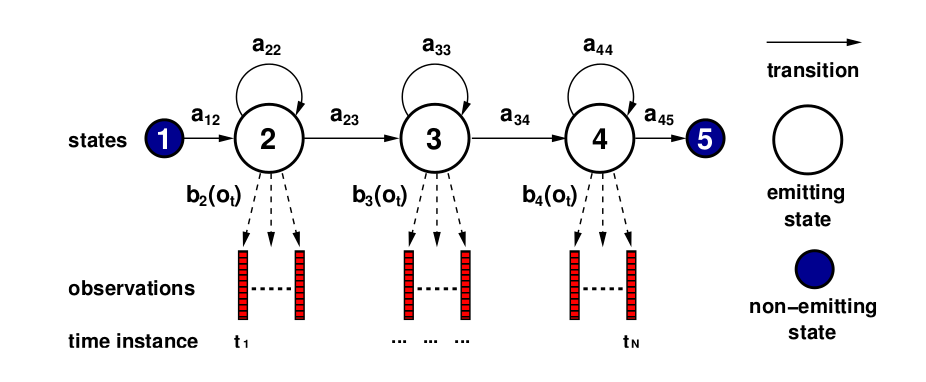
\includegraphics[width=240pt]{HMM.png}
\end{figure}
$M$ means all the parameters on the HMM, including the transition probability $a_{ij}$ and $\mu_j$ and $\Sigma_j$ for the Guassian distribution $b_j$.\\
EM is a iterative method, $M_k$ means the result we get in the kth iteration.\\
H is the hypothesis that our data is indeed from a HMM.
\end{frame}

\begin{frame}
\begin{figure}
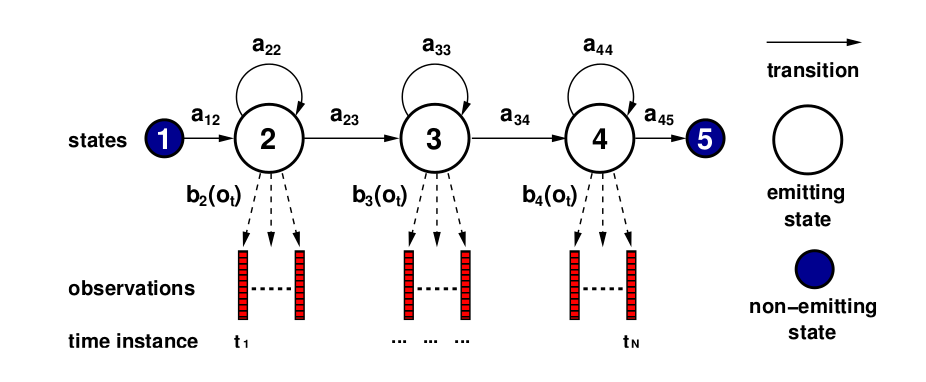
\includegraphics[width=240pt]{HMM.png}
\end{figure}
We can easily see that
\begin{equation}
P(w|H,M)=\prod_{t}a_{w_{t-1}w_t}
\end{equation}
\end{frame}

\begin{frame}
\frametitle{The Object function}
\begin{itemize}
	\item Now we apply MLE to HMM, so we maximize the log likelyhood function, 
	\begin{equation}{\label{1}}
	\begin{split}
		logp(O|H,M) &= log \sum_{w}p(O|w,H,M)p(w|H,M) \\
		& = log \sum_{w}a_{w_0w_1}
			\prod_{t}a_{w_{t-1}w_t}b_{w_t}(o_t) 
	\end{split}
	\end{equation}
	where $w$ is the state sequence, and $O$ is the observance.
	\item However, equation \ref{1} is untractable, for we have to enumerate all $w$.
\end{itemize}
\end{frame}

\begin{frame}
\frametitle{Some simplification}
\begin{itemize}
	\item For the remaining part of this tutorial, I will omit the omnipresent hypothesis $H$. \
	\item We will now assume that $b(o)$ is Guassian (instead of Guassian Mixture) for simplicity.
\end{itemize}
\end{frame}

\begin{frame}
\frametitle{Jensen's Inequality}
\framesubtitle{push the log in}
\begin{block}{Jensen's Inequality}
If $X$ is a random variable and $\varphi$ is a convex function.
Then $\varphi(E[X]) \leq E[\varphi(X)]$.
\begin{figure}
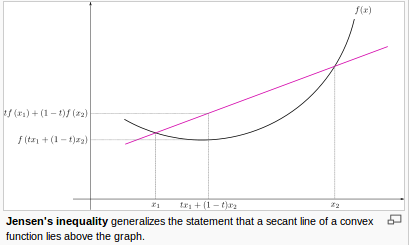
\includegraphics[width=200pt]{jensen.png}
\end{figure}
\end{block}
\end{frame}

\begin{frame}
\frametitle{Apply the Jensen inequailty}
Note:$logp(O|M)=log\sum_wp(O,w|M)$\\
Remembering that $-log$ is convex and $\varphi(E[X]) \leq E[\varphi(X)]$, we can select any $q$. So
\begin{equation}{\label{2}}
\begin{split}
	logp(O|M) &= log \sum_{w}\frac{q(w) p(O,w|M)}{q(w)} \\
				& \geq <logp(O,w|M)>_{q(w)} + H(q(w)) 
\end{split}
\end{equation}
Where $	<f(x)>_{P(x)} = \sum_x f(x)P(x)$and$H(P(x)) = - \sum_x{P(x)logP(x)}$.
It can be shown \cite{Dempster} that the inequality \ref{2} \alert{becomes an equality} when $q(w) = P(w|O,M)$.
\end{frame}

\begin{frame}
\frametitle{How do we choose $M_{k+1}$}
\framesubtitle{The anxiliary function}
Equation \ref{2} gives a lower bound for $P(O|M_{k+1})$ by setting $q(w) = p(w|O,\hat{M}_k)$
\begin{equation}
logp(O|M_{k+1}) \geq <logp(O,w|M_{k+1})>_{p(w|O,\hat{M}_k)} + H(P(w|O,\hat{M}_k))
\end{equation}
Now, let us define the auxiliary function:
\begin{equation}
Q_{ML}(M_{k+1};\hat{M}_k) = <logp(O,w|M_{k+1})>_{p(w|O,\hat{M}_k)}
\end{equation}
So, out task is now clearly to maximize the anxiliary function with respect to $M_{k+1}$, and suppose we find the $\hat{M}_{k+1}$. With the result of \cite{Dempster} and the fact that $Q_{ML}(\hat{M}_{k+1};\hat{M_k}) \geq Q_{ML}(\hat{M}_k;\hat{M_k})$, we are able to proof \alert{the lowerbond of $P(O|\hat{M}_{k+1})$ is greater than $P(O|\hat{M}_{k})$}.
\end{frame}

\begin{frame}
\frametitle{Proof for $P(O|\hat{M}_{k+1}) \geq P(O|\hat{M}_{k})$}

\begin{theorem}
$P(O|\hat{M}_{k+1})$ is greater than $P(O|\hat{M}_{k})$, if $\hat{M}_{k+1}$ maximizes the anxiliary function.
\end{theorem}

\begin{proof}
From the assumption we have 
$Q_{ML}(\hat{M}_{k+1};\hat{M_k}) \geq Q_{ML}(\hat{M}_k;\hat{M_k})$
We add a constant to both sides
$Q_{ML}(\hat{M}_{k+1};\hat{M_k}) + H(P(w|O,\hat{M}_k)) \geq Q_{ML}(\hat{M}_k;\hat{M_k}) + H(P(w|O,\hat{M}_k))$ \\
Now we know that the r.h.s is exactly $logP(O|\hat{M}_{k})$ and the l.h.s is a lowerbond of $P(O|\hat{M}_{k+1})$, which gives the result.
\end{proof}
\end{frame}

\begin{frame}
\frametitle{What do E and M mean?}
From 
\begin{equation}
logp(O|M_{k+1}) \geq <logp(O,w|M_{k+1})>_{p(w|O,\hat{M}_k)} + H(P(w|O,\hat{M}_k))
\end{equation}
we now know that in order to maximize the lowerbound, we only need to maximize the auxiliary function $Q_{ML}(M_{k+1};\hat{M}_k) = <logp(O,w|M_{k+1})>_ {p(w|O,\hat{M}_k)}$.\\
Now we can see the outline for the E-M algorithm. We use the state distribution from the last iteration to \alert{estimate} the performance of this new iteration, and then \alert{maximize} it.
\begin{block}{A joke}
We want to maximize $(3+2)x, x \leq 5$.\\
In the E step, we compute 3+2.\\
In the M step, we maximize $5x$ with $x \leq 5$.
\end{block}
\end{frame}

\begin{frame}
\frametitle{E:Unfold the anxiliary function}
\begin{equation}
\begin{split}
Q_{ML}(M_{k+1};\hat{M}_{k}) = \sum_w logp(O,w|M_{k+1})p(w|O,\hat{M}_k) \\
                            = \sum_w log(a_{w_0w_1}\prod_ta_{w_{t-1}w_t}b_{w_t}(o_t)) P(w|O, \hat{M}_k) \\
Q_{ML}(M_{k+1};\hat{M}_{k}) = \sum_{t,j} \gamma_j(t)logb_j(o_t)+\sum_{t,i,j}\varepsilon_{ij}(t)loga_{ij}
\end{split}                 
\end{equation}
Where $\gamma_j(t) = P(w_t=j|O,\hat{M}_k)$ and $\varepsilon_{ij}(t) = P(w_{t-1}=i,w_t=j|O,\hat{M}_k)$. And the transistion is simply via take each $a$ and $b$ out and add all out their cooresponding $w$.
\end{frame}

\begin{frame}
\frametitle{E:The Forward-Backward Algorithm}
To calculate $\gamma_j$ and $\varepsilon_{ij}$, we need to calculate $\alpha_j(t) = p(o_{1-t}, w_t=j|\hat{M}_k)$ and $\beta_j(t)=p(o_{t+1-T}|w_t=j, \hat{M}_k)$
They can be calculated efficiently:
\begin{equation}
\begin{split}
\alpha_j(t) = (\sum_{i=2}^{N-1}\alpha_i(t-1)a_{ij})b_j(o_t) \\
\beta_j(t) = \sum_{i=2}^{N-1}a_{ji}b_i(o_{t+1})\beta_i(t+1)
\end{split}
\end{equation}
\end{frame}

\begin{frame}
\frametitle{E:Use $\alpha$ and $\beta$ to get $\gamma$ and $\varepsilon$ }
\begin{theorem}
$\gamma_j(t)= \frac{\alpha_j(t) \beta_j(t)}{p(O|\hat{M}_k)}$ and 
$\varepsilon_{ij}(t) = \frac{\alpha_i(t-1) a_{ij} b_j(o_t) \beta_j(t)}{p(O|\hat{M}_k)}$
\end{theorem}
\begin{proof}
I only proof the first equation. Plug the definition in.\\
$\frac{\alpha_j(t) \beta_j(t)}{p(O|\hat{M}_k)} = 
\frac{p(o_{1-t}, w_t=j|\hat{M}_k)p(o_{t+1-T}|w_t=j, \hat{M}_k)}{p(O|\hat{M}_k)}$ \\
$= \frac{p(o_{1-t}|w_t=j, \hat{M}_k)p(w_t=j|\hat{M}_k)p(o_{t+1-T}|w_t=j, \hat{M}_k)}{p(O|\hat{M}_k)}$ \\
note the condition $w_t=j$ makes the two probability independent.
$=\frac{p(o_{1-T}|w_t=j,\hat{M}_k)p(w_t=j|\hat{M}_k)}{p(O|\hat{M}_k)}$ \\
$=p(w_t=j|O,\hat{M}_k)$
\end{proof}
\end{frame}

\begin{frame}
\frametitle{M:Use the Lagrange Multiplier}
Having got the $\gamma$ and $\varepsilon$, we finally could try to maximize 
\begin{equation}
Q_{ML}(M_{k+1};\hat{M}_{k}) = \sum_{t,j} \gamma_j(t)logb_j(o_t)+\sum_{t,i,j}\varepsilon_{ij}(t)loga_{ij}
\end{equation}
First let's consider $a_{i*}$, now we should maxmize $\sum_{t,j} \varepsilon_{ij}(t)loga_{ij}$ subject to $\sum_j a_{ij} = 1$
\end{frame}
\begin{block}{The Lagrange Multiplier}
We want to maximize $f(x,y)$ subject $g(x,y) = c$.\\
Let $\Lambda(x, y \lambda) = f(x,y) + \lambda (g(x,y)-c)$.Then if $(x_0, y_0)$is a maximum of the original $f$, there exists $(x_0,y_0,\lambda_0)$ is a stationary point for the $\Lambda$ function.\\
\begin{figure}[L]
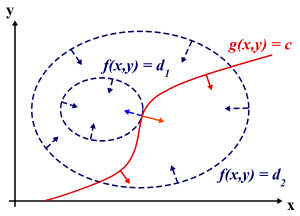
\includegraphics[width=130pt]{Lagrange.png}
\end{figure}
The contour lines of f and g touch when the tangent vectors of the contour lines are parallel. Since the gradient of a function is perpendicular to the contour lines, this is the same as saying that the gradients of f and g are parallel. 
\end{block}

\begin{frame}
\begin{block}{The Lagrange Multiplier}
So $\nabla_{x,y}f =  - \lambda \nabla_{x,y}g$.\\
Combining with the constraint, we get $\nabla_{x,y,\lambda}\Lambda = 0$
\end{block}
Now we apply the Lagrange Multiplier method to maxmize $\sum_{t,j} \varepsilon_{ij}(t)loga_{ij}$ subject to $\sum_j a_{ij} = 1$. We get(I'll do the computing on the blackboard)
\begin{equation}
\hat{a}_{ij} = \frac{\sum^{T}_{t=2}\varepsilon_{ij}(t)}{\sum^{T}_{t=1}\gamma_i(t)}
\end{equation}
\end{frame}

\begin{frame}
Now we maximize the other component $\sum_{t,j} \gamma_j(t)logb_j(o_t)$.We set $G(\mu_j, \Sigma_j) = \sum_{t} \gamma_j(t)logb_j(o_t)$. And we maximize it by solving $\frac{\partial G}{\partial \mu_j}=0$. \\
With the experience of MLE for Guassian distribution in the introduction part, this should be rather easy, I omit the computing here.
\begin{equation}
\hat{\mu_j} = \frac{\sum_t(\gamma_j(t)o_t)}{\sum_t\gamma_j(t)}
\end{equation}
Sorry that I didn't compute the $\hat{\Sigma_j}$.
\end{frame}



\begin{frame}
\frametitle{Extending to GMM}
Extending single Guassian to Guassian Mixture is not part of this tutorial, and these two slices are poorly written. I encourage reader to refer to PRML \$9.2 for knowledge of GMM, then you can use the technique introduced here to extend to GMM yourself!
\end{frame}
\begin{frame}
\frametitle{Extending to GMM}
To get the value of the Guassians, we first need to introduce sub-states by extending $w$.
	\begin{equation}
	\begin{split}
		Q_{ML}(M_{k+1};\hat{M}_{k}) = &\sum_w logp(O,w|M_{k+1})p(w|O,\hat{M}_k) \\
                            = &\sum_w log(a_{w_0w_1}\prod_ta_{w_{t-1}w_t}c_{w_td_t}b_{w_td_t}(o_t)) P(w|O, \hat{M}_k) \\
	\end{split}
	\end{equation}
Where $c$ is weight of the component.
And now we can apply the Lagrange Multiplier method.
\end{frame}

\begin{frame}
\frametitle{Extending to GMM}
If we set
\begin{equation}
\gamma_{jm}(t)=\frac{\sum_{i=2}^{N-1}\alpha_i(t-1)a_{ij}c_{jm}b_{jm}(o_t)\beta_j(t)}{p(O|M_k)}
\end{equation}
Then
\begin{equation}
\begin{split}
\hat{c}_{jm}=\frac{\sum_t\gamma_{jm}(t)}{\sum_{m,t}\gamma_{jm}(t)} \\
\hat{\mu}_{jm}=\frac{\sum_t\gamma_{jm}(t)o_t}{\sum_{t}\gamma_{jm}(t)}
\end{split}
\end{equation}
\end{frame}


\section*{Bibliography}
\begin{frame}%[allowframebreaks] % add this if you have more papers to cite than fit on a slide.
\frametitle{Bibliography}

\begin{thebibliography}{Tantau, 2007}
\bibitem[KaiYu, 2006]{Kai}
Adaptive Training for Large Vocabulary Continuous Speech Recognition

\bibitem[A.P.Dempster, 1977]{Dempster}
Maximum likelihood from incomplete data via the EM algorithm


\end{thebibliography}
\end{frame}
\end{document}
